\documentclass[10pt]{article}
\usepackage{geometry}                % See geometry.pdf to learn the layout options. There are lots.
\geometry{letterpaper}                   % ... or a4paper or a5paper or ... 
%\geometry{landscape}                % Activate for for rotated page geometry
\usepackage[parfill]{parskip}    % Activate to begin paragraphs with an empty line rather than an indent
\usepackage[cm]{fullpage}
\usepackage{graphicx}
\usepackage{amssymb}
\usepackage[margin=20pt, font=small, labelfont=sc, labelsep=endash]{caption}
\usepackage{subfig}
\usepackage{multirow}
%\usepackage{pstricks, pst-node,pst-tree}


\title{Analysis of loadings}
\author{Wesley Brooks}
\date{}                                           % Activate to display a given date or no date

\usepackage{Sweave}
\begin{document}
\setkeys{Gin}{width=0.9\textwidth}    %make figures a bit wider than the Sweave default.
\maketitle


















\begin{figure}[h!]
    \begin{center}
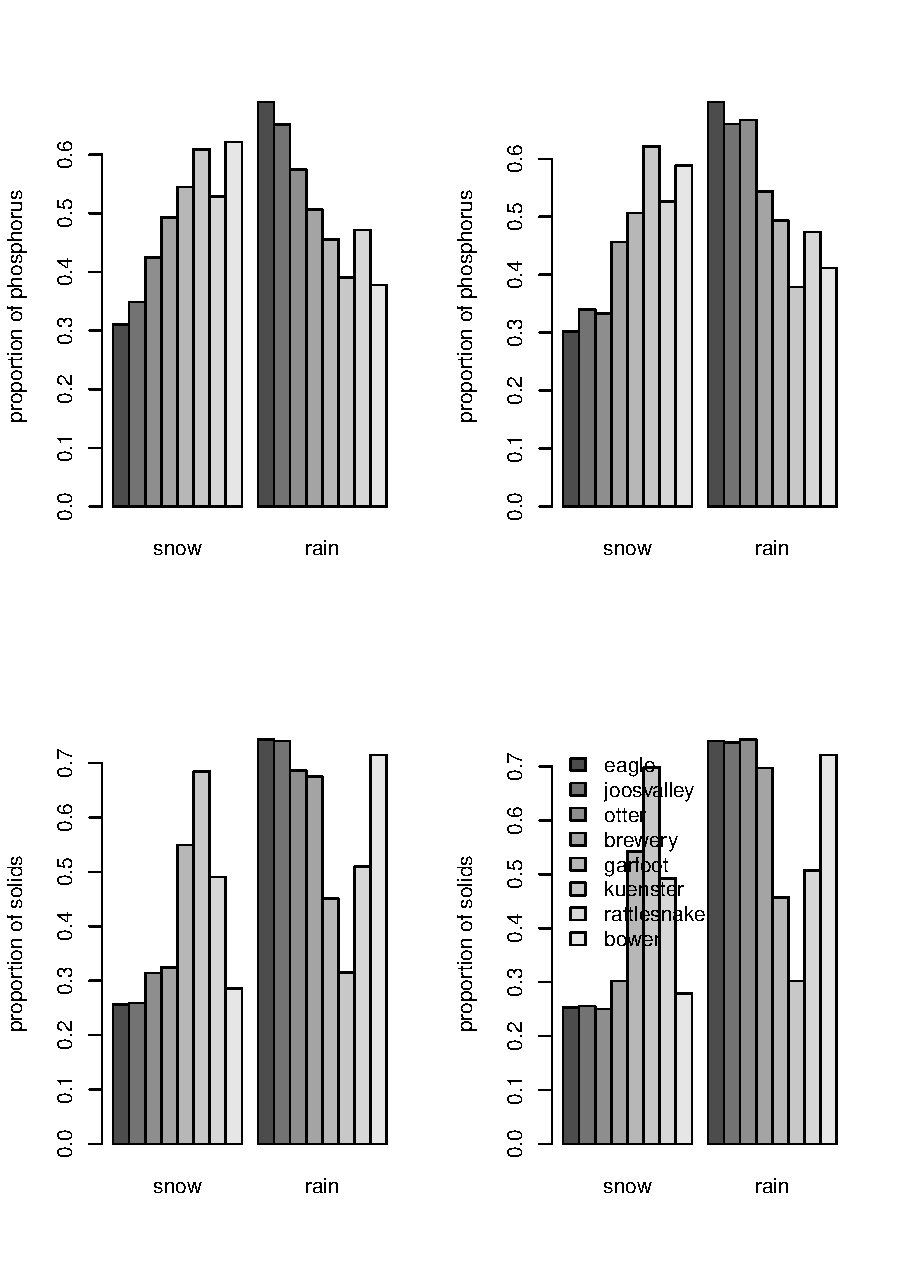
\includegraphics{loadings-fig2}
    \end{center}
    \vspace{-10mm}
    \caption{Cumulative storm loadings at the four creeks.\label{bars}}
\end{figure}










%Boxplots of the contribution from individual storm events
\begin{figure}[h]
    \setkeys{Gin}{width=1\textwidth}    %make figures a bit wider than the Sweave default.
    \begin{center}
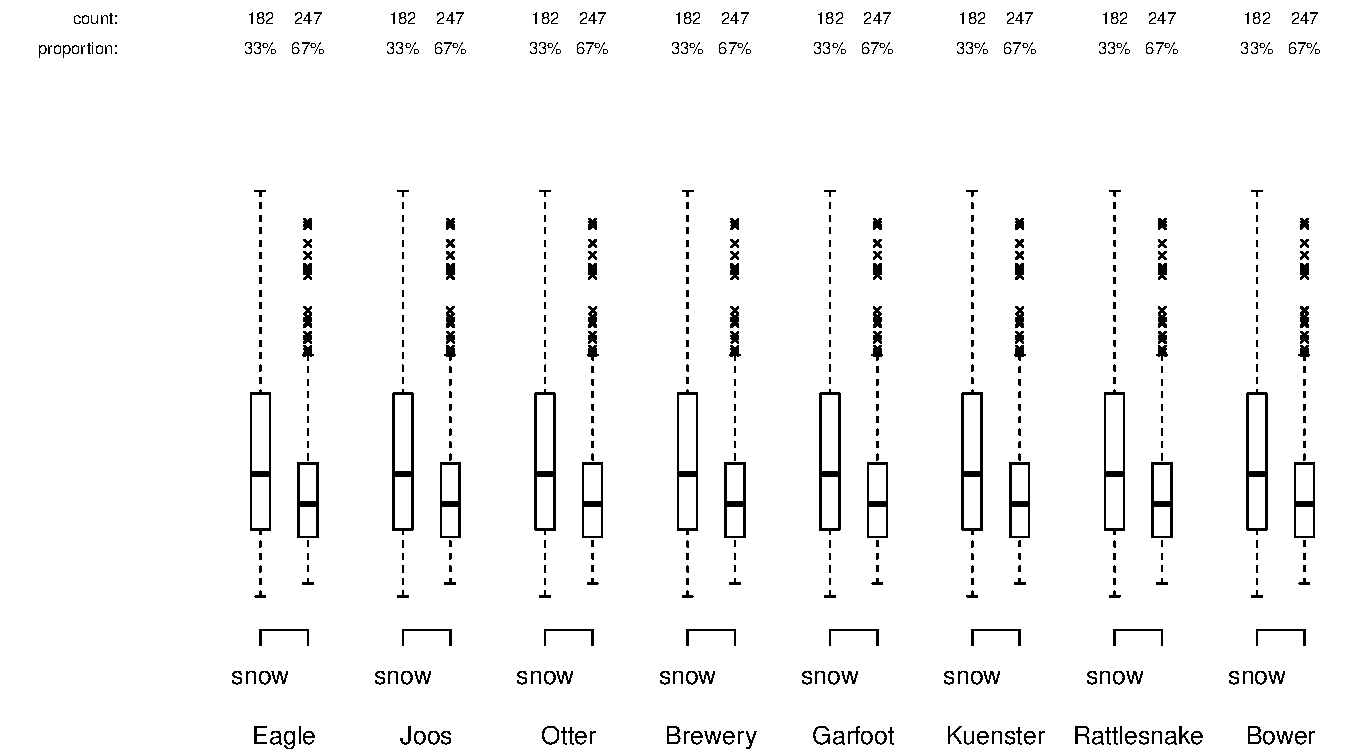
\includegraphics{loadings-boxplot_stot}
    \vspace{15mm}
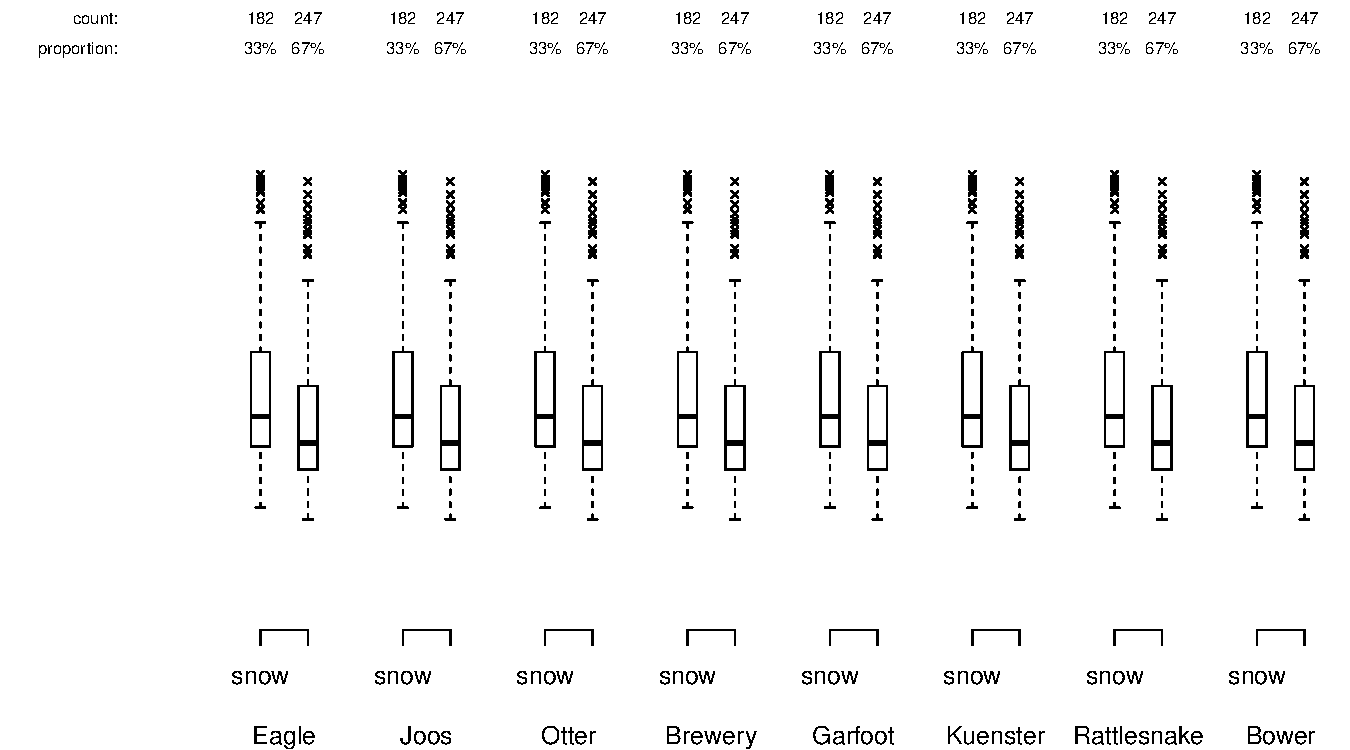
\includegraphics{loadings-boxplot_ptot}
    \caption{Boxplots showing the sediment and phosphorus load produced by individual events at all four streams.\label{boxplots}}
    \end{center}
\end{figure}










    
    



\section{Goal}
Stream health is threatened by high sediment and phosphorus loads, which are carried into the streams by runoff from the surrounding landscape. It has been shown previously\cite{Danz:2010} that the phosphorus and sediment loads in Wisconsin are not evenly distributed in time - rather, most of the annual loading arrives during two pulses: one in early spring, associated with the melting of the winter snowpack, and the other in midsummer, at the same time as the most intense summer thunderstorms.\\

In this study, we define loading "events" that can span multiple days of continuous runoff. Our goal is to then characterize the events that produce the greatest loading, in order to inform management practices that aim to improve stream health by reducing sediment and phosphorus loads. Our ultimate goal is a mathematical model of stream loading based on some easily-interpretable covariates. Ideally, we will arrive at a global model for all the sites in the study. The alternative are a collection of local models that seem to describe only the specific sites at which they are calibrated.\\

\section{Data}
\paragraph{Description}
The data in this report comes from eight Wisconsin streams that were monitored (with some gaps in data collection) between 1989 and 2009. The streams and the period during which each was monitored are in Table \ref{table:dates}, except that the phosphorus loading was not measured at Brewery Creek from October 1999 onward.\\

\begin{table}[h]
\begin{center}
\begin{tabular}{r c l}
        \textbf{Stream}  & \textbf{Events} & \textbf{Years}\\
        Eagle & 429 & 1991-1994, 2003-2007\\
        Joos Valley & 473 & 1990-1994, 2002-2007\\
        Otter & 424 & 1990-1997, 2000-2002\\
        Brewery & 670 & 1985, 1990-1998, 2000-2001\\
        Garfoot & 527 & 1985, 1990-1993, 1995-1998\\
        Kuenster & 218 & 1992-1995\\
        Rattlesnake & 170 & 1991-1994\\
        Bower & 373 & 1990-1994, 2006-2009\\
    \end{tabular}
    \label{table:dates}
\end{center}
\end{table}

Each entry in our data set represents one loading event. Events are defined based on the hydrograph - an event begins when the flow rises from a base level toward a peak, and ends when the flow falls back to its new base level. A computer program called Rainmaker was used to separate the total stream flow into base flow and storm flow components. The hydrograph separation is done by analyzing the beginning and ending base flows and the peak storm flow for each event. The storm flow input that drives each event can come from rainfall, from melting snow, or from some combination of the two.

Two kinds of load are measured for each event - the sediment load and the phosphorus load. The load from each event can be divided into two components: the base flow component and the storm flow component. The two components refer, respectively, to the load carried by the stream's base flow and that carried by the additional storm flow pulse. Rainmaker separates the two components based on the hydrograph.\\

Not all of the data can be collected for each event. For instance, rainfall is measured only when the ground is free of snow, because snow interferes with the rain gauges. And the amount of snowmelt is estimated by multiplying the snow's water content by the change in snow depth during a warm snap, which is inaccurate when additional snow falls during the event. Broadly, there is one set of measurements that are made during rainfall-driven events and a different set of measurements that are made during snowmelt-driven events. Because of this, the two types of event are modeled separately. Furthermore, compared to the data about events that are rainfall-driven, the data about events that are snowmelt-driven is of lower quality. That's because: the accuracy of the stream gauge is reduced by ice on the stream, the winter rainfall, snow depth, and water content are not measured locally (snow data tends (or is it always?) to come from the nearest large airport.) It would be surprising if the accuracy of models for snowmelt-driven loading were comparable to that of models for rainfall-driven loading.\\

All else being equal, a stream that drains a larger area should have a greater flow, and should carry a greater load of sediment and phosphorus. For this reason, the sediment and phosphorus loads were divided by the drainage area to get the sediment and phosphorus yields. The yields will be the output from our models.\\

We augmented the data with some antecedent values that we thought could possibly affect the loadings produced during an event. These were the base flow one day before the event, the two-day antecedent mean temperature, the maximum temperature over the two days before the event, and the range between the two-day antecedent max and min temperatures.\\

Some of the data were measured at a gauge station on each stream - these were the stream gauge, local rainfall (including intensity and duration), and the concentrations of sediment and phosphorus (the concentrations were multiplied by the stream flow to get the loadings.) Other data such as rainfall, snowfall, snow depth, snow water content, and air temperature were measured by the National Weather Service (NWS) at a permanent weather station. We downloaded these data from a database maintained by the NWS. Finally we have some metadata that describes our data at the watershed level: the drainage area, the average stream slope, and the land use composition.\\


\paragraph{Exploratory Analysis}
The first task was to determine how loads are distributed between snowmelt-driven and rainfall-driven events. The total loads from each kind of event are tabulated in Tables \ref{tab:stot} (sediment) and \ref{tab:ptot} (phosphorus). Figure \ref{bars} presents the same information as the tables, while Figure \ref{boxplots} also compares the load from indivudual snowmelt- and rainfall-driven events. In general, more of the load of both phosphorus and sediment is from rainfall-driven events, but at Garfoot and Kuenster more of the both kinds of load came from snowmelt-driven events. At all sites except Garfoot and Kuenster, snowmelt-driven events contributed a larger proportion of phosphorus loading than of sediment loading (and at Garfoot and Kuenster, difference between the proportions was small.) At most sites the difference between the proportion of sediment load produced by snowmelt-driven events and the proportion of phosphorus load produced by snowmelt-driven events was less than ten percentage points, but at Bower the difference was about 34 percentage points. This suggests that melting snow carries proportionally more phosphorus than does rainfall-runoff, which might be the case if the the phosphorus is from animal poop that accumulates on fallen snow, while the sediment comes from dirt that is mainly trapped under the snowpack.\\

\subparagraph{Rainfall-driven events}
We investigated dividing the snow-free seasons into early and late subseasons, separating the two on May 15th of each year. If vegetation serves to hold the soil together, and to increase both evapotranspiration and infiltration, then erosion may be more common early in the spring before most of the summer's vegetation appears. If so, the relationship between rainfall and the stream's loading might change during the summer.\\

The investigation was done by making linear models to describe the sediment and phosphorus loading during the two subseasons and comparing them to a single model fit to the entire snow-free period. Because the split makes the model more flexible, it will certainly improve the model's fit - the question is whether that improvement is enough to justify making the model more complex. At all four streams, the model improvement was statistically significant but too small to matter (the split models explained about 1\%-2\% more of the loads). We will not use the split in the rest of the analysis.\\

% latex table generated in R 2.14.1 by xtable 1.6-0 package
% Thu Feb 02 19:31:50 2012
\begin{table}[ht]
\begin{center}
\begin{tabular}{lcc}
  & snowmelt-driven & rainfall-driven \\ 
  \hline
Eagle & 27.0\% & 73.0\% \\ 
  Joos & 26.9\% & 73.1\% \\ 
  Otter & 35.4\% & 64.6\% \\ 
  Brewery & 32.8\% & 67.2\% \\ 
  Garfoot & 55.6\% & 44.4\% \\ 
  Kuenster & 68.5\% & 31.5\% \\ 
  Rattlesnake & 48.9\% & 51.1\% \\ 
  Bower & 28.8\% & 71.2\% \\ 
  \end{tabular}
\caption{Proportion of total suspended solids loading contributed by each type of event}
\label{tab:stot}
\end{center}
\end{table}
% latex table generated in R 2.14.1 by xtable 1.6-0 package
% Thu Feb 02 19:31:50 2012
\begin{table}[ht]
\begin{center}
\begin{tabular}{lcc}
  & snowmelt-driven & rainfall-driven \\ 
  \hline
Eagle & 32.8\% & 67.2\% \\ 
  Joos & 36.4\% & 63.6\% \\ 
  Otter & 46.5\% & 53.5\% \\ 
  Brewery & 49.6\% & 50.4\% \\ 
  Garfoot & 55.2\% & 44.8\% \\ 
  Kuenster & 61.1\% & 38.9\% \\ 
  Rattlesnake & 52.6\% & 47.4\% \\ 
  Bower & 62.9\% & 37.1\% \\ 
  \end{tabular}
\caption{Proportion of total phosphorus loading contributed by each type of event}
\label{tab:ptot}
\end{center}
\end{table}
\subparagraph{Snowmelt-driven events}
Since sediment and phosphorus are carried into streams by runoff, it makes intuitive sense that the amount of loading during an event should depend on the amount of runoff during that event. In the case of rainfall-driven loading events, it is straightforward to use rain gauges to measure the amount of water entering the stream system. In the case of snowmelt-driven loading events, though, it is not easy to measure how much water melts out of the snowpack, especially when there is also additional snow falling at the same time. There is a subset of events for which we are able to estimate the amount of melting water: Those are the events when we have a measurement of the snow's water content and of the snow depth both before and after the event, and no additional snow falls during the event.\\

We would like to make a model that uses the available event data to describe the amount of sediment and phosphorus loading. In order to use our estimate of the snowmelt as a predictor of loading, we must ignore the snowmelt-driven events for which we cannot estimate the snowmelt. In order to determine whether that will bias our results, we first look at the overall proportion of loading that is provided by the events we will not be modeling.\\


We can also compare the size of events that will be ignored versus the size of events that will be modeled. The p-values of the tests comparing the sediment and phosphorus loads from each event at each stream are tabulated in table \ref{tab:ignored_test1}.\\

% latex table generated in R 2.14.1 by xtable 1.6-0 package
% Thu Feb 02 19:31:50 2012
\begin{table}[ht]
\begin{center}
\begin{tabular}{lcc}
  & Sediment & Phosphorus \\ 
  \hline
Eagle & 0.002 & 0.026 \\ 
  Joos & 0.002 & 0.004 \\ 
  Otter & 0.833 & 0.491 \\ 
  Brewery & 0.779 & 0.444 \\ 
  Garfoot & 0.573 & 0.157 \\ 
  Kuenster & 0.302 & 0.623 \\ 
  Rattlesnake & 0.835 & 0.699 \\ 
  Bower & 0.017 & 0.014 \\ 
  \end{tabular}
\caption{P-values of tests of the difference in the load contributed by ignored and modeled snowmelt-driven events.}
\label{tab:ignored_test1}
\end{center}
\end{table}
Finally, we compare the dates when the ignored events occured to the dates when the modeled events occured. The p-values for the test at each stream are tabulated in Table \ref{tab:ignored_test2}.\\

% latex table generated in R 2.14.1 by xtable 1.6-0 package
% Thu Feb 02 19:31:50 2012
\begin{table}[ht]
\begin{center}
\begin{tabular}{lc}
  & p-value \\ 
  \hline
Eagle & 0.942 \\ 
  Joos & 0.278 \\ 
  Otter & 0.234 \\ 
  Brewery & 0.591 \\ 
  Garfoot & 0.121 \\ 
  Kuenster & 0.169 \\ 
  Rattlesnake & 0.047 \\ 
  Bower & 0.443 \\ 
  \end{tabular}
\caption{P-values of tests of the difference in the date of modeled snowmelt-driven events compared to the ignored events.}
\label{tab:ignored_test2}
\end{center}
\end{table}
in most cases there is not a statistically significant difference in size or date between the events for which \verb+total_water+ is known, and those for which it is not. It therefore looks like the model results won't be badly biased by ignoring the events for which we don't have an estimate of the snowmelt.\\

\subparagraph{Major events}
Over the course of the monitoring period, the majority of the total load (both of sediment and of phosphorus) was carried during just a few major events. Just 10\% of the events carried between 73.1\% (at Otter) and 97.1\% (at Bower) of the total sediment load; the same events produced between 64.6\% (at Otter) and 88\% (at Joos) of the total phosphorus load.\\




\begin{table}[h] \small
    \begin{center}
    \begin{tabular}{lrl}
    \textbf{Sediment} & $R^2$ & Model terms \\
    \hline
\multirow{7}{*}{Eagle} & 0.515 & theisen\\ 
 & 0.769 & theisen + antecedent\_qbase\_quantile\\ 
 & 0.781 & theisen + antecedent\_qbase\_quantile + p15max\\ 
 & 0.786 & theisen + antecedent\_qbase\_quantile + p15max + duration\\ 
 & 0.808 & theisen + antecedent\_qbase\_quantile + p15max + duration + ap\_1day\\ 
 & 0.814 & theisen + antecedent\_qbase\_quantile + p15max + duration + ap\_1day + p30max\\ 
\vspace{2mm}\\ \multirow{5}{*}{Joos} & 0.501 & theisen\\ 
 & 0.718 & theisen + antecedent\_qbase\_quantile\\ 
 & 0.745 & theisen + antecedent\_qbase\_quantile + p15max\\ 
 & 0.755 & theisen + antecedent\_qbase\_quantile + p15max + ap\_3day\\ 
\vspace{2mm}\\ \multirow{4}{*}{Otter} & 0.508 & theisen\\ 
 & 0.798 & theisen + antecedent\_qbase\_quantile\\ 
 & 0.808 & theisen + antecedent\_qbase\_quantile + ap\_1day\\ 
\vspace{2mm}\\ \multirow{5}{*}{Brewery} & 0.494 & theisen\\ 
 & 0.711 & theisen + antecedent\_qbase\_quantile\\ 
 & 0.727 & theisen + antecedent\_qbase\_quantile + antecedent\_tmean\\ 
 & 0.744 & theisen + antecedent\_qbase\_quantile + antecedent\_tmean + p10max\\ 
\vspace{2mm}\\ \multirow{5}{*}{Garfoot} & 0.444 & theisen\\ 
 & 0.665 & theisen + antecedent\_qbase\_quantile\\ 
 & 0.678 & theisen + antecedent\_qbase\_quantile + p30max\\ 
 & 0.702 & theisen + antecedent\_qbase\_quantile + p30max + ei\\ 
\vspace{2mm}\\ \multirow{3}{*}{Kuenster} & 0.408 & theisen\\ 
 & 0.768 & theisen + antecedent\_qbase\_quantile\\ 
\vspace{2mm}\\ \multirow{5}{*}{Rattlesnake} & 0.479 & antecedent\_qbase\_quantile\\ 
 & 0.759 & antecedent\_qbase\_quantile + theisen\\ 
 & 0.778 & antecedent\_qbase\_quantile + theisen + ap\_5day\\ 
 & 0.791 & antecedent\_qbase\_quantile + theisen + ap\_5day + ap\_1day\\ 
\vspace{2mm}\\ \multirow{4}{*}{Bower} & 0.348 & antecedent\_qbase\_quantile\\ 
 & 0.737 & antecedent\_qbase\_quantile + theisen\\ 
 & 0.745 & antecedent\_qbase\_quantile + theisen + ap\_5day\\ 
\vspace{2mm}\\ \multirow{9}{*}{Aggregate} & 0.414 & theisen\\ 
 & 0.688 & theisen + antecedent\_qbase\_quantile\\ 
 & 0.705 & theisen + antecedent\_qbase\_quantile + slope\\ 
 & 0.711 & theisen + antecedent\_qbase\_quantile + slope + p15max\\ 
 & 0.724 & theisen + antecedent\_qbase\_quantile + slope + p15max + ei\\ 
 & 0.726 & theisen + antecedent\_qbase\_quantile + slope + p15max + ei + num\_events\\ 
 & 0.728 & theisen + antecedent\_qbase\_quantile + slope + p15max + ei + num\_events + p5max\\ 
 & 0.73 & theisen + antecedent\_qbase\_quantile + slope + p15max + ei + num\_events + p5max + p30max\\ 
\vspace{2mm}\\     \end{tabular}
    \caption{Results of variable selection for a model of sediment loading from rainfall-driven events\label{sed_r_square_nosnow}}
    \end{center}
\end{table}

\begin{table}[h] \small
    \begin{center}
    \begin{tabular}{lrl}
    \textbf{Phosphorus} & $R^2$ & Model terms \\
    \hline
\multirow{6}{*}{Eagle} & 0.58 & theisen\\ 
 & 0.772 & theisen + antecedent\_qbase\_quantile\\ 
 & 0.783 & theisen + antecedent\_qbase\_quantile + p15max\\ 
 & 0.795 & theisen + antecedent\_qbase\_quantile + p15max + ap\_1day\\ 
 & 0.8 & theisen + antecedent\_qbase\_quantile + p15max + ap\_1day + p30max\\ 
\vspace{2mm}\\ \multirow{5}{*}{Joos} & 0.544 & theisen\\ 
 & 0.747 & theisen + antecedent\_qbase\_quantile\\ 
 & 0.764 & theisen + antecedent\_qbase\_quantile + p15max\\ 
 & 0.776 & theisen + antecedent\_qbase\_quantile + p15max + ap\_3day\\ 
\vspace{2mm}\\ \multirow{4}{*}{Otter} & 0.486 & theisen\\ 
 & 0.801 & theisen + antecedent\_qbase\_quantile\\ 
 & 0.807 & theisen + antecedent\_qbase\_quantile + ap\_1day\\ 
\vspace{2mm}\\ \multirow{4}{*}{Brewery} & 0.609 & theisen\\ 
 & 0.752 & theisen + antecedent\_qbase\_quantile\\ 
 & 0.763 & theisen + antecedent\_qbase\_quantile + ap\_3day\\ 
\vspace{2mm}\\ \multirow{5}{*}{Garfoot} & 0.545 & theisen\\ 
 & 0.67 & theisen + antecedent\_qbase\_quantile\\ 
 & 0.704 & theisen + antecedent\_qbase\_quantile + nws\_prec\\ 
 & 0.716 & theisen + antecedent\_qbase\_quantile + nws\_prec + ap\_5day\\ 
\vspace{2mm}\\ \multirow{4}{*}{Kuenster} & 0.44 & theisen\\ 
 & 0.764 & theisen + antecedent\_qbase\_quantile\\ 
 & 0.798 & theisen + antecedent\_qbase\_quantile + ap\_3day\\ 
\vspace{2mm}\\ \multirow{4}{*}{Rattlesnake} & 0.366 & theisen\\ 
 & 0.61 & theisen + antecedent\_qbase\_quantile\\ 
 & 0.665 & theisen + antecedent\_qbase\_quantile + ap\_5day\\ 
\vspace{2mm}\\ \multirow{7}{*}{Bower} & 0.517 & antecedent\_qbase\_quantile\\ 
 & 0.757 & antecedent\_qbase\_quantile + nws\_prec\\ 
 & 0.789 & antecedent\_qbase\_quantile + nws\_prec + theisen\\ 
 & 0.811 & antecedent\_qbase\_quantile + nws\_prec + theisen + tmin\\ 
 & 0.821 & antecedent\_qbase\_quantile + nws\_prec + theisen + tmin + tmean\\ 
 & 0.826 & antecedent\_qbase\_quantile + nws\_prec + theisen + tmin + tmean + ap\_5day\\ 
\vspace{2mm}\\ \multirow{9}{*}{Aggregate} & 0.395 & theisen\\ 
 & 0.615 & theisen + antecedent\_qbase\_quantile\\ 
 & 0.62 & theisen + antecedent\_qbase\_quantile + p15max\\ 
 & 0.63 & theisen + antecedent\_qbase\_quantile + p15max + ei\\ 
 & 0.636 & theisen + antecedent\_qbase\_quantile + p15max + ei + tmin\\ 
 & 0.643 & theisen + antecedent\_qbase\_quantile + p15max + ei + tmin + tmax\\ 
 & 0.646 & theisen + antecedent\_qbase\_quantile + p15max + ei + tmin + tmax + slope\\ 
 & 0.647 & theisen + antecedent\_qbase\_quantile + p15max + ei + tmin + tmax + slope + p30max\\ 
\vspace{2mm}\\     \end{tabular}
    \caption{Results of variable selection for a model of phosphorus loading from rainfall-driven events\label{phos_r_square_nosnow}}
    \end{center}
\end{table}


\begin{table}[h] \small
    \begin{center}
    \begin{tabular}{lrl}
    \textbf{Sediment} & $R^2$ & Model terms \\
    \hline
\multirow{4}{*}{Eagle} & 0.246 & antecedent\_qbase\_quantile\\ 
 & 0.4 & antecedent\_qbase\_quantile + tmax\\ 
 & 0.594 & antecedent\_qbase\_quantile + tmax + total\_water\\ 
\vspace{2mm}\\ \multirow{6}{*}{Joos} & 0.217 & tmax\\ 
 & 0.405 & tmax + total\_water\\ 
 & 0.512 & tmax + total\_water + antecedent\_qbase\_quantile\\ 
 & 0.555 & tmax + total\_water + antecedent\_qbase\_quantile + sin\_julian\\ 
 & 0.583 & tmax + total\_water + antecedent\_qbase\_quantile + sin\_julian + num\_days\\ 
\vspace{2mm}\\ \multirow{5}{*}{Otter} & 0.262 & tmax\\ 
 & 0.294 & tmax + antecedent\_qbase\_quantile\\ 
 & 0.494 & tmax + antecedent\_qbase\_quantile + total\_water\\ 
 & 0.531 & tmax + antecedent\_qbase\_quantile + total\_water + cos\_julian\\ 
\vspace{2mm}\\ \multirow{3}{*}{Brewery} & 0.33 & antecedent\_qbase\_quantile\\ 
 & 0.478 & antecedent\_qbase\_quantile + num\_days\\ 
\vspace{2mm}\\ \multirow{5}{*}{Garfoot} & 0.272 & num\_days\\ 
 & 0.455 & num\_days + antecedent\_qbase\_quantile\\ 
 & 0.607 & num\_days + antecedent\_qbase\_quantile + total\_water\\ 
 & 0.644 & num\_days + antecedent\_qbase\_quantile + total\_water + nws\_snow\\ 
\vspace{2mm}\\ \multirow{4}{*}{Kuenster} & 0.451 & melt\_water\\ 
 & 0.56 & melt\_water + num\_days\\ 
 & 0.639 & melt\_water + num\_days + sin\_julian\\ 
\vspace{2mm}\\ \multirow{4}{*}{Rattlesnake} & 0.189 & num\_days\\ 
 & 0.196 & num\_days + antecedent\_tmax\\ 
 & 0.197 & num\_days + antecedent\_tmax + cos\_julian\\ 
\vspace{2mm}\\ \multirow{7}{*}{Bower} & 0.422 & total\_water\\ 
 & 0.476 & total\_water + nws\_snow\\ 
 & 0.56 & total\_water + nws\_snow + antecedent\_tmean\\ 
 & 0.631 & total\_water + nws\_snow + antecedent\_tmean + num\_days\\ 
 & 0.689 & total\_water + nws\_snow + antecedent\_tmean + num\_days + antecedent\_qbase\_quantile\\ 
 & 0.718 & total\_water + nws\_snow + antecedent\_tmean + num\_days + antecedent\_qbase\_quantile + nws\_prec\\ 
\vspace{2mm}\\ \multirow{10}{*}{Aggregate} & 0.139 & num\_days\\ 
 & 0.284 & num\_days + antecedent\_qbase\_quantile\\ 
 & 0.313 & num\_days + antecedent\_qbase\_quantile + tmax\\ 
 & 0.371 & num\_days + antecedent\_qbase\_quantile + tmax + nws\_prec\\ 
 & 0.392 & num\_days + antecedent\_qbase\_quantile + tmax + nws\_prec + slope\\ 
 & 0.416 & num\_days + antecedent\_qbase\_quantile + tmax + nws\_prec + slope + nws\_snow\\ 
 & 0.435 & num\_days + antecedent\_qbase\_quantile + tmax + nws\_prec + slope + nws\_snow + cos\_julian\\ 
 & 0.484 & num\_days + antecedent\_qbase\_quantile + tmax + nws\_prec + slope + nws\_snow + cos\_julian + total\_water\\ 
 & 0.492 & num\_days + antecedent\_qbase\_quantile + tmax + nws\_prec + slope + nws\_snow + cos\_julian + total\_water + sin\_julian\\ 
\vspace{2mm}\\     \end{tabular}
    \caption{Results of variable selection for a model of sediment loading from snowmelt-driven events.\label{sed_r_square_snow}}
    \end{center}
\end{table}



\begin{table}[h] \small
    \begin{center}
    \begin{tabular}{lrl}
    \textbf{Phosphorus} & $R^2$ & Model terms \\
    \hline
\multirow{4}{*}{Eagle} & 0.218 & antecedent\_qbase\_quantile\\ 
 & 0.41 & antecedent\_qbase\_quantile + tmax\\ 
 & 0.609 & antecedent\_qbase\_quantile + tmax + total\_water\\ 
\vspace{2mm}\\ \multirow{5}{*}{Joos} & 0.228 & tmax\\ 
 & 0.286 & tmax + nws\_prec\\ 
 & 0.398 & tmax + nws\_prec + num\_days\\ 
 & 0.49 & tmax + nws\_prec + num\_days + antecedent\_qbase\_quantile\\ 
\vspace{2mm}\\ \multirow{5}{*}{Otter} & 0.29 & tmax\\ 
 & 0.434 & tmax + total\_water\\ 
 & 0.557 & tmax + total\_water + antecedent\_qbase\_quantile\\ 
 & 0.597 & tmax + total\_water + antecedent\_qbase\_quantile + cos\_julian\\ 
\vspace{2mm}\\ \multirow{5}{*}{Brewery} & 0.152 & num\_days\\ 
 & 0.308 & num\_days + antecedent\_qbase\_quantile\\ 
 & 0.34 & num\_days + antecedent\_qbase\_quantile + sin\_julian\\ 
 & 0.419 & num\_days + antecedent\_qbase\_quantile + sin\_julian + nws\_prec\\ 
\vspace{2mm}\\ \multirow{5}{*}{Garfoot} & 0.237 & num\_days\\ 
 & 0.402 & num\_days + total\_water\\ 
 & 0.462 & num\_days + total\_water + antecedent\_qbase\_quantile\\ 
 & 0.501 & num\_days + total\_water + antecedent\_qbase\_quantile + nws\_snow\\ 
\vspace{2mm}\\ \multirow{3}{*}{Kuenster} & 0.552 & total\_water\\ 
 & 0.669 & total\_water + nws\_snow\\ 
\vspace{2mm}\\ \multirow{4}{*}{Rattlesnake} & 0.244 & num\_days\\ 
 & 0.254 & num\_days + antecedent\_tmax\\ 
 & 0.257 & num\_days + antecedent\_tmax + cos\_julian\\ 
\vspace{2mm}\\ \multirow{6}{*}{Bower} & 0.36 & total\_water\\ 
 & 0.553 & total\_water + antecedent\_qbase\_quantile\\ 
 & 0.667 & total\_water + antecedent\_qbase\_quantile + num\_days\\ 
 & 0.754 & total\_water + antecedent\_qbase\_quantile + num\_days + antecedent\_tmean\\ 
 & 0.776 & total\_water + antecedent\_qbase\_quantile + num\_days + antecedent\_tmean + nws\_snow\\ 
\vspace{2mm}\\ \multirow{9}{*}{Aggregate} & 0.139 & num\_days\\ 
 & 0.298 & num\_days + antecedent\_qbase\_quantile\\ 
 & 0.338 & num\_days + antecedent\_qbase\_quantile + tmax\\ 
 & 0.427 & num\_days + antecedent\_qbase\_quantile + tmax + total\_water\\ 
 & 0.434 & num\_days + antecedent\_qbase\_quantile + tmax + total\_water + nws\_prec\\ 
 & 0.452 & num\_days + antecedent\_qbase\_quantile + tmax + total\_water + nws\_prec + nws\_snow\\ 
 & 0.464 & num\_days + antecedent\_qbase\_quantile + tmax + total\_water + nws\_prec + nws\_snow + sin\_julian\\ 
 & 0.475 & num\_days + antecedent\_qbase\_quantile + tmax + total\_water + nws\_prec + nws\_snow + sin\_julian + cos\_julian\\ 
\vspace{2mm}\\     \end{tabular}
    \caption{Results of variable selection for a model of phosphorus loading from snowmelt-driven events.\label{phos_r_square_snow}}
    \end{center}
\end{table}


\section{Analysis}

\subsection{Variable selection}
In order to make a model of the load carried by the stream, we need to select the predictor variables that have explanatory power. We used stepwise regression with the Bayesian Information Criterion (BIC) to screen the potential predictor variables. We begin the selection with an intercept-only model, and at each step we add or remove one variable. The variable that is added or removed is the one whose addition or removal will do the most to reduce the BIC. If no such variable is found, then selection is considered complete.\\

\paragraph{Rainfall-driven events} The predictors that survived the screening at each stream are listed in Table \ref{nosnow_predictor_list}. The variables are listed in the order of their importance to the model.\\

\begin{table}[h!]\small
    \begin{center}
    \begin{tabular}{ll}
        \textbf{Solids} & \\
        \hspace{5mm} Eagle: & theisen, antecedent\_qbase\_quantile, p15max, duration, ap\_1day, p30max\\
        \hspace{5mm} Joos: & theisen, antecedent\_qbase\_quantile, p15max, ap\_3day\\
        \hspace{5mm} Otter: & theisen, antecedent\_qbase\_quantile, ap\_1day\\
        \hspace{5mm} Brewery: & theisen, antecedent\_qbase\_quantile, antecedent\_tmean, p10max\\
        \hspace{5mm} Garfoot: & theisen, antecedent\_qbase\_quantile, p30max, ei\\
        \hspace{5mm} Kuenster: & theisen, antecedent\_qbase\_quantile\\
        \hspace{5mm} Rattlesnake: & antecedent\_qbase\_quantile, theisen, ap\_5day, ap\_1day \\
        \hspace{5mm} Bower: & antecedent\_qbase\_quantile, theisen, ap\_5day\\
        \hspace{5mm} Aggregate: & theisen, antecedent\_qbase\_quantile, slope, p15max, ei, num\_events, p5max, p30max
    \vspace{2mm}\\
        \textbf{Phosphorus} & \\
        \hspace{5mm} Eagle: & theisen, antecedent\_qbase\_quantile, p15max, ap\_1day, p30max\\
        \hspace{5mm} Joos: & theisen, antecedent\_qbase\_quantile, p15max, ap\_3day\\
        \hspace{5mm} Otter: & theisen, antecedent\_qbase\_quantile, ap\_1day\\
        \hspace{5mm} Brewery: & theisen, antecedent\_qbase\_quantile, ap\_3day\\
        \hspace{5mm} Garfoot: & theisen, antecedent\_qbase\_quantile, nws\_prec, ap\_5day\\
        \hspace{5mm} Kuenster: & theisen, antecedent\_qbase\_quantile, ap\_3day\\
        \hspace{5mm} Rattlenake: & theisen, antecedent\_qbase\_quantile, ap\_5day\\
        \hspace{5mm} Bower: & antecedent\_qbase\_quantile, nws\_prec, theisen, tmin, tmean, ap\_5day\\
        \hspace{5mm} Aggregate: & theisen, antecedent\_qbase\_quantile, p15max, ei, tmin, tmax, slope, p30max\\
    \end{tabular}
    \caption{The most important variables in the models for rainfall-driven loading. The variables are ordered by their importance to the model of the load. \label{nosnow_predictor_list}}
    \end{center}
\end{table}

In each case, the two most important predictors are the theisen rainfall and the antecedent baseflow. Using just those two predictors results in an $R^2$ greater than 0.7 in most models (see Tables \ref{sed_r_square_nosnow} and \ref{phos_r_square_nosnow}.) Since the antecedent baseflow is considered an indicator of how much water is in the watershed before each event, we conclude that the amount of sediment and phosphorus washed into a stream by each event is mainly a function of the quantity of water moving through the system. At Brewery Creek, the intensity of rainfall is a more important predictor than the total quantity of rain.\\

The performance of the global (aggregate) model is quite good: with just two predictors (sediment: \Sexp{paste(as$ranked[1:2], sep=", ")}, phosphorus: \Sexp{paste(ap$ranked[1:2], sep=", ")}) the $\text{R}^2$ is \Sexp{round(as$R2[2], 2)} and \Sexp{round(ap$R2[2], 2)}, respectively. In the case of sediment, the next-most-important predictor is the stream slope. Including it in the model pushes the $\text{R}^2$ to \Sexp{round(ap$R2[3], 2)}.\\

\paragraph{Snowmelt-driven events} We had less success modeling the loading produced by the snowmelt-driven events. The predictors that survived the screening process were different from stream to stream and those variables that did survive at most sites weren't always selected in the same order (like they were for the rainfall-driven events). What's more, the models for snowmelt-driven events were less accurate than for rainfall-driven events, ranging in $R^2$ from 0.24 to 0.53, with most in the 0.45 range.\\

At most sites, the most important predictor was a temperature measurement, either the maximum or the mean temperature during the loading event. The antecedent baseflow also appears to be important at most sites. It seems likely that, as in the case of rainfall-driven events, the loading is driven by the quantity of water that moves through the watershed during the event.\\

\begin{table}[h!]\small
    \begin{center}
    \begin{tabular}{ll}
        \textbf{Solids} & \\
        \hspace{5mm} Eagle: & antecedent\_qbase\_quantile, tmax, total\_water\\
        \hspace{5mm} Joos: & tmax, total\_water, antecedent\_qbase\_quantile, sin\_julian, num\_days\\
        \hspace{5mm} Otter: & tmax, antecedent\_qbase\_quantile, total\_water, cos\_julian\\
        \hspace{5mm} Brewery: & antecedent\_qbase\_quantile, num\_days\\
        \hspace{5mm} Garfoot: & num\_days, antecedent\_qbase\_quantile, total\_water, nws\_snow\\
        \hspace{5mm} Kuenster: & melt\_water, num\_days, sin\_julian\\
        \hspace{5mm} Rattlesnake: & num\_days, antecedent\_tmax, cos\_julian \\
        \hspace{5mm} Bower: & total\_water, nws\_snow, antecedent\_tmean, num\_days, antecedent\_qbase\_quantile, nws\_prec\\
        \hspace{5mm} Aggregate: & num\_days, antecedent\_qbase\_quantile, tmax, nws\_prec, slope, nws\_snow, cos\_julian, total\_water, sin\_julian
    \vspace{2mm}\\
        \textbf{Phosphorus} & \\
        \hspace{5mm} Eagle: & antecedent\_qbase\_quantile, tmax, total\_water\\
        \hspace{5mm} Joos: & tmax, nws\_prec, num\_days, antecedent\_qbase\_quantile\\
        \hspace{5mm} Otter: & tmax, total\_water, antecedent\_qbase\_quantile, cos\_julian\\
        \hspace{5mm} Brewery: & num\_days, antecedent\_qbase\_quantile, sin\_julian, nws\_prec\\
        \hspace{5mm} Garfoot: & num\_days, total\_water, antecedent\_qbase\_quantile, nws\_snow\\
        \hspace{5mm} Kuenster: & total\_water, nws\_snow\\
        \hspace{5mm} Rattlesnake: & num\_days, antecedent\_tmax, cos\_julian\\
        \hspace{5mm} Bower: & total\_water, antecedent\_qbase\_quantile, num\_days, antecedent\_tmean, nws\_snow\\
        \hspace{5mm} Aggregate: & num\_days, antecedent\_qbase\_quantile, tmax, total\_water, nws\_prec, nws\_snow, sin\_julian, cos\_julian\\
    \end{tabular}
    \caption{The most important variables in the models for snowmelt-driven loading. The variables are ordered by their importance to the model of the load. \label{snow_predictor_list}}
    \end{center}
\end{table}

\section{Conclusions}
We have an accurate global model that describes the loading that will result from a rainstorm, based just on the base flow before the storm and on the amount of rain that falls during the storm. Antecedent base flow is a measurement of how much water is in the watershed before a storm and any new water comes as rainfall, so it seems that the sediment and phosphorus loads are driven mainly by the quantity of water moving through the watershed. The stream slope also seems to be important; that could be because steeper slopes give surface water less time to infiltrate and therefore increase the intensity of a rainfall event.\\

We have not yet found an accurate way to model the amount of load during a snowmelt-driven event but we have seen that the air temperature (which drives snowmelt), the antecedent base flow, and the amount of additional precipitation are important predictors for those events.\\

Most of the annual loading seems to be produced by a few major events. If the goal is to reduce the impact of sediment and phosphorus loading on stream health, then something must be done to mitigate the impact of those major events. Figures \ref{cdf-s} and \ref{cdf-p} make it look like the majority of the ranfall-driven loading comes from storms that drop at least two inches of rain. Mitigating the effect of large storms will probably require slowing the water's movement through the watershed - for instance, by impounding runoff before it can flow into the creeks. A further analysis should look at the frequency of big storms in order to get an idea of how quickly impounded water must be dealt with in order to be ready for the next event.\\


\begin{figure}
    \begin{center}
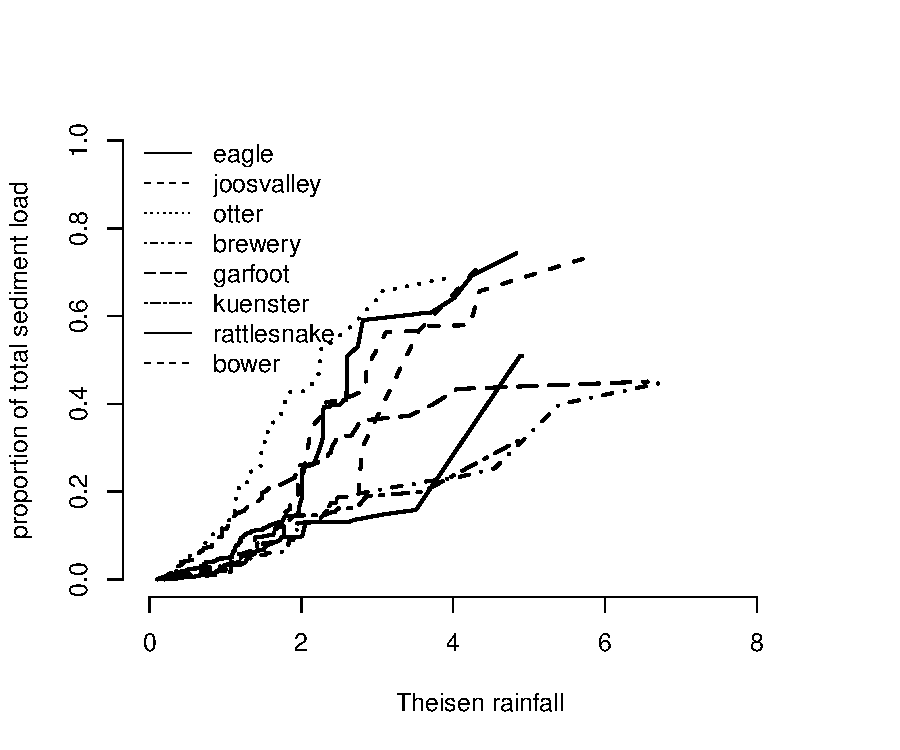
\includegraphics{loadings-figure2}
    \end{center}
    \caption{Proportion of the total sediment load contributed by rainfall events up to the size shown. Snowmelt-driven events are excluded.\label{cdf-p}}
\end{figure}

\begin{figure}
    \begin{center}
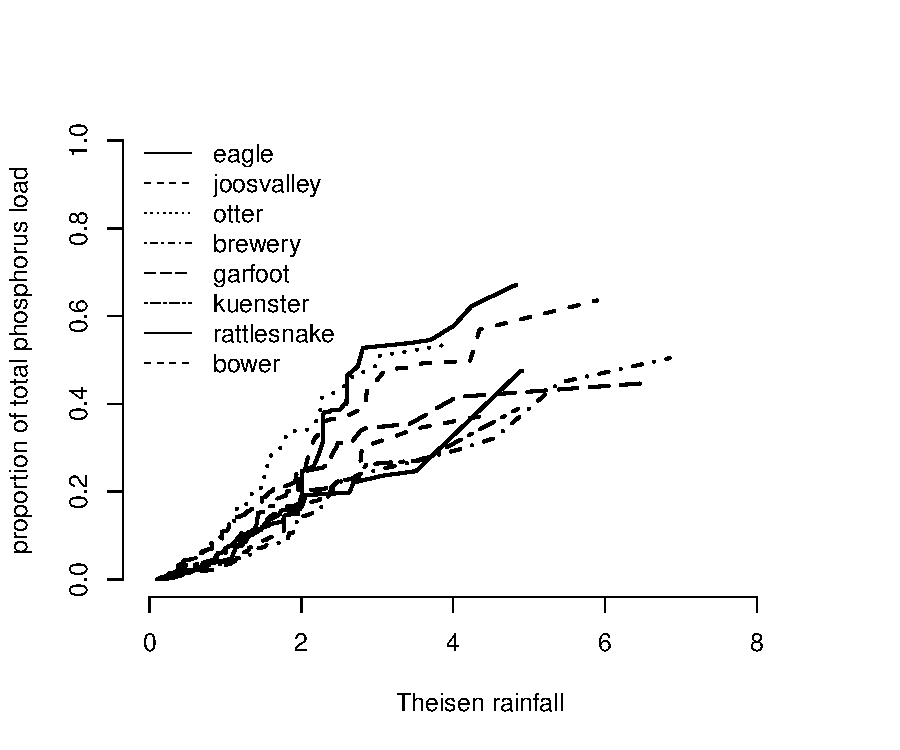
\includegraphics{loadings-figure3}
    \end{center}
    \caption{Proportion of the total phosphorus load contributed by rainfall events up to the size shown. Snowmelt-driven events are excluded.\label{cdf-s}}
\end{figure}

\begin{figure}
    \begin{center}
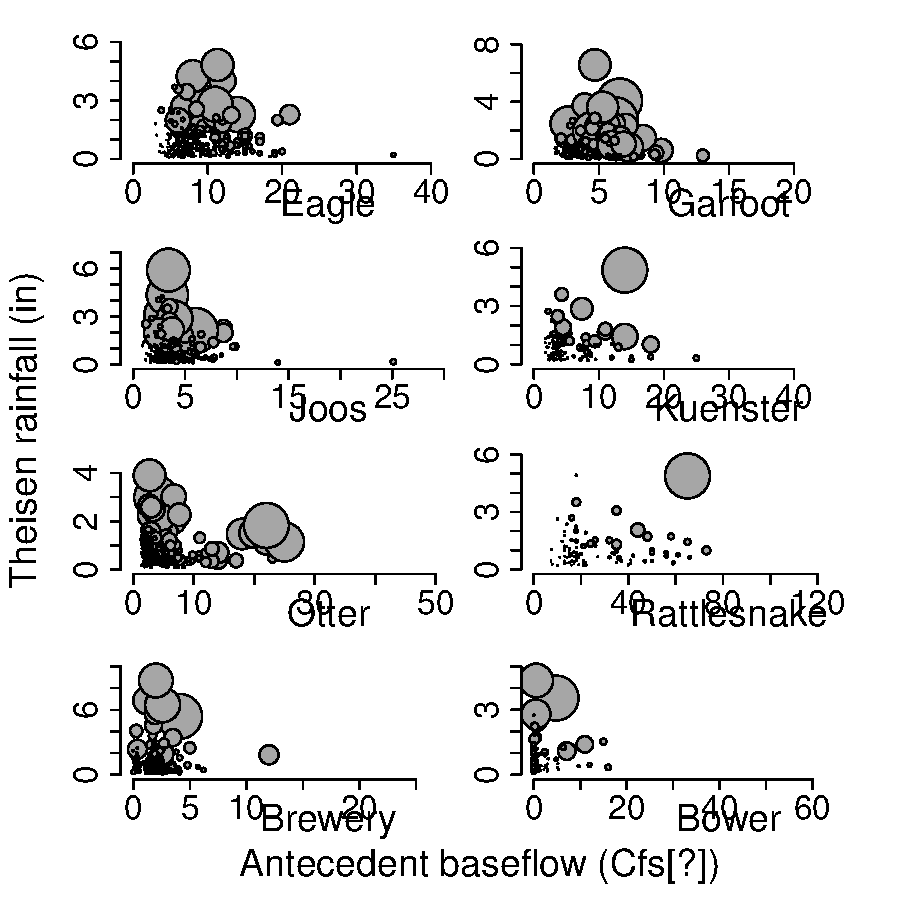
\includegraphics{loadings-figure4}
    \end{center}
    \caption{Antecedent base flow is the horizontal axis; theisen rainfall is the vertical axis. Each dot represents one event. The size of the dot shows the total sediment load contributed by that event. \label{bubbles}}
\end{figure}


\bibliographystyle{plain}
\bibliography{../references/loadings}

\end{document}
